\subsubsection*{Regularização}

Quando se modela uma arquitetura de redes neurais pode se chegar em três casos, sendo eles: subajuste (underfit), balanceado (optimal) e sobreajuste (overfit). O sobreajuste é quando no treinamento o modelo acerta as classes porém nos testes não, isso mostra uma dificuldade em generalizar as características. Já o subajuste não consegue pontuar bem em nenhum caso mostrando que o conjunto de dados de treinamento está pequeno para detectar padrões. Por outro lado,  o balanceado é quando produz resultados bons tanto no conjunto de dados de treinamento quanto no de testes \cite{Alzubaidi2021, computation11030052}.

\begin{figure}[H]
	\caption{Gráficos mostrando subajuste, balanceado e sobreajuste respectivamente} 
	\centering % para centralizarmos a figura
	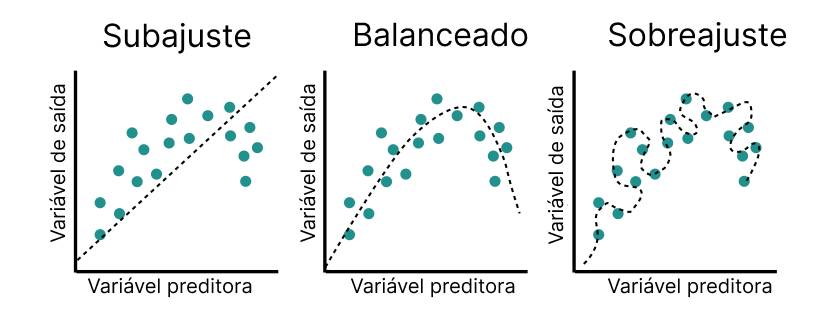
\includegraphics[width=15cm]{figures/fittings.png} % leia abaixo
	\legend{Fonte: \citeonline{educative2022overfitting}}
	\label{fig:arquitetura_cnn}
\end{figure}
% \footnote{Nota de rodapé}
% \footnote[Numero do rodapé]{Nota de rodapé}



